%\section*{Results}
\section*{Identifying Potential Saline Stress Responsive Genes in Rice}
\label{sec.case}

This section presents a case study, applying the approach introduced in 
\hyperref[sec.framework]{the Workflow} section, to identify genes in
\textit{Oryza sativa} that respond to saline stress.
\vspace{0.5cm}

The RNA-seq data are available from the
GEO database \cite{clough2016gene} (accession
number GSE98455). It corresponds to $n_0=57\,845$ gene
expression profiles of shoot tissues measured for control and
salt conditions in $m=92$ accessions of the Rice Diversity Panel 1~\cite{eizenga2014registration},
with $r=2$ biological replicates. A total of $p=3 $ phenotypic traits
are used: shoot $K$ content, root biomass, and shoot biomass. These
traits were measured for the same $92$ genotypes, under control and
treatment conditions, and can be found in the supplementary
information for~\cite{campbell2017allelic}.

\subsection*{A. Data Pre-processing}

DESeq2 normalization is applied to the raw data and the biological
replicates are averaged. Genes exhibiting low variance are
identified as those with ratio of upper quantile to lower quantile
smaller than $1.5$ and are removed from the normalized data. Genes
with low expression, corresponding to those having more than $80\%$
samples with values smaller than $10$, are also removed. After this
filtering process a total of $n_1 = 9\,414$ genes are kept for further analysis.
\vspace{0.5cm}

From the Log Fold Change matrix $L_0$, genes whose difference between
upper quantile and lower quantile is greater than $0.25$ are
removed. Therefore, the resulting matrix $L_1$ contains the log ratios
of $n_2 = 8\,928$ genes. The logarithmic ratios of the phenotypic data,
for the $92$ accessions and the $3$ traits, are also computed.

\subsection*{B. Construction of the Co-expression Network}

The Log Fold Change matrix $L_1$ is used to compute the corresponding
similarity matrix.  For this network, it is observed that $\beta=3$ is
the smallest integer such that the $R^2 \geq 0.8
$. Figure~\ref{fig:beta} depicts the degree distribution of the
similarity matrix (left) and the degree distribution of the adjacency
matrix (right), which is the degree distribution of a scale-free
network with $R^2 = 0.8$ with $\beta = 3$.
\vspace{0.5cm}

%figure 2
\begin{figure}[htbp]
  \centering
    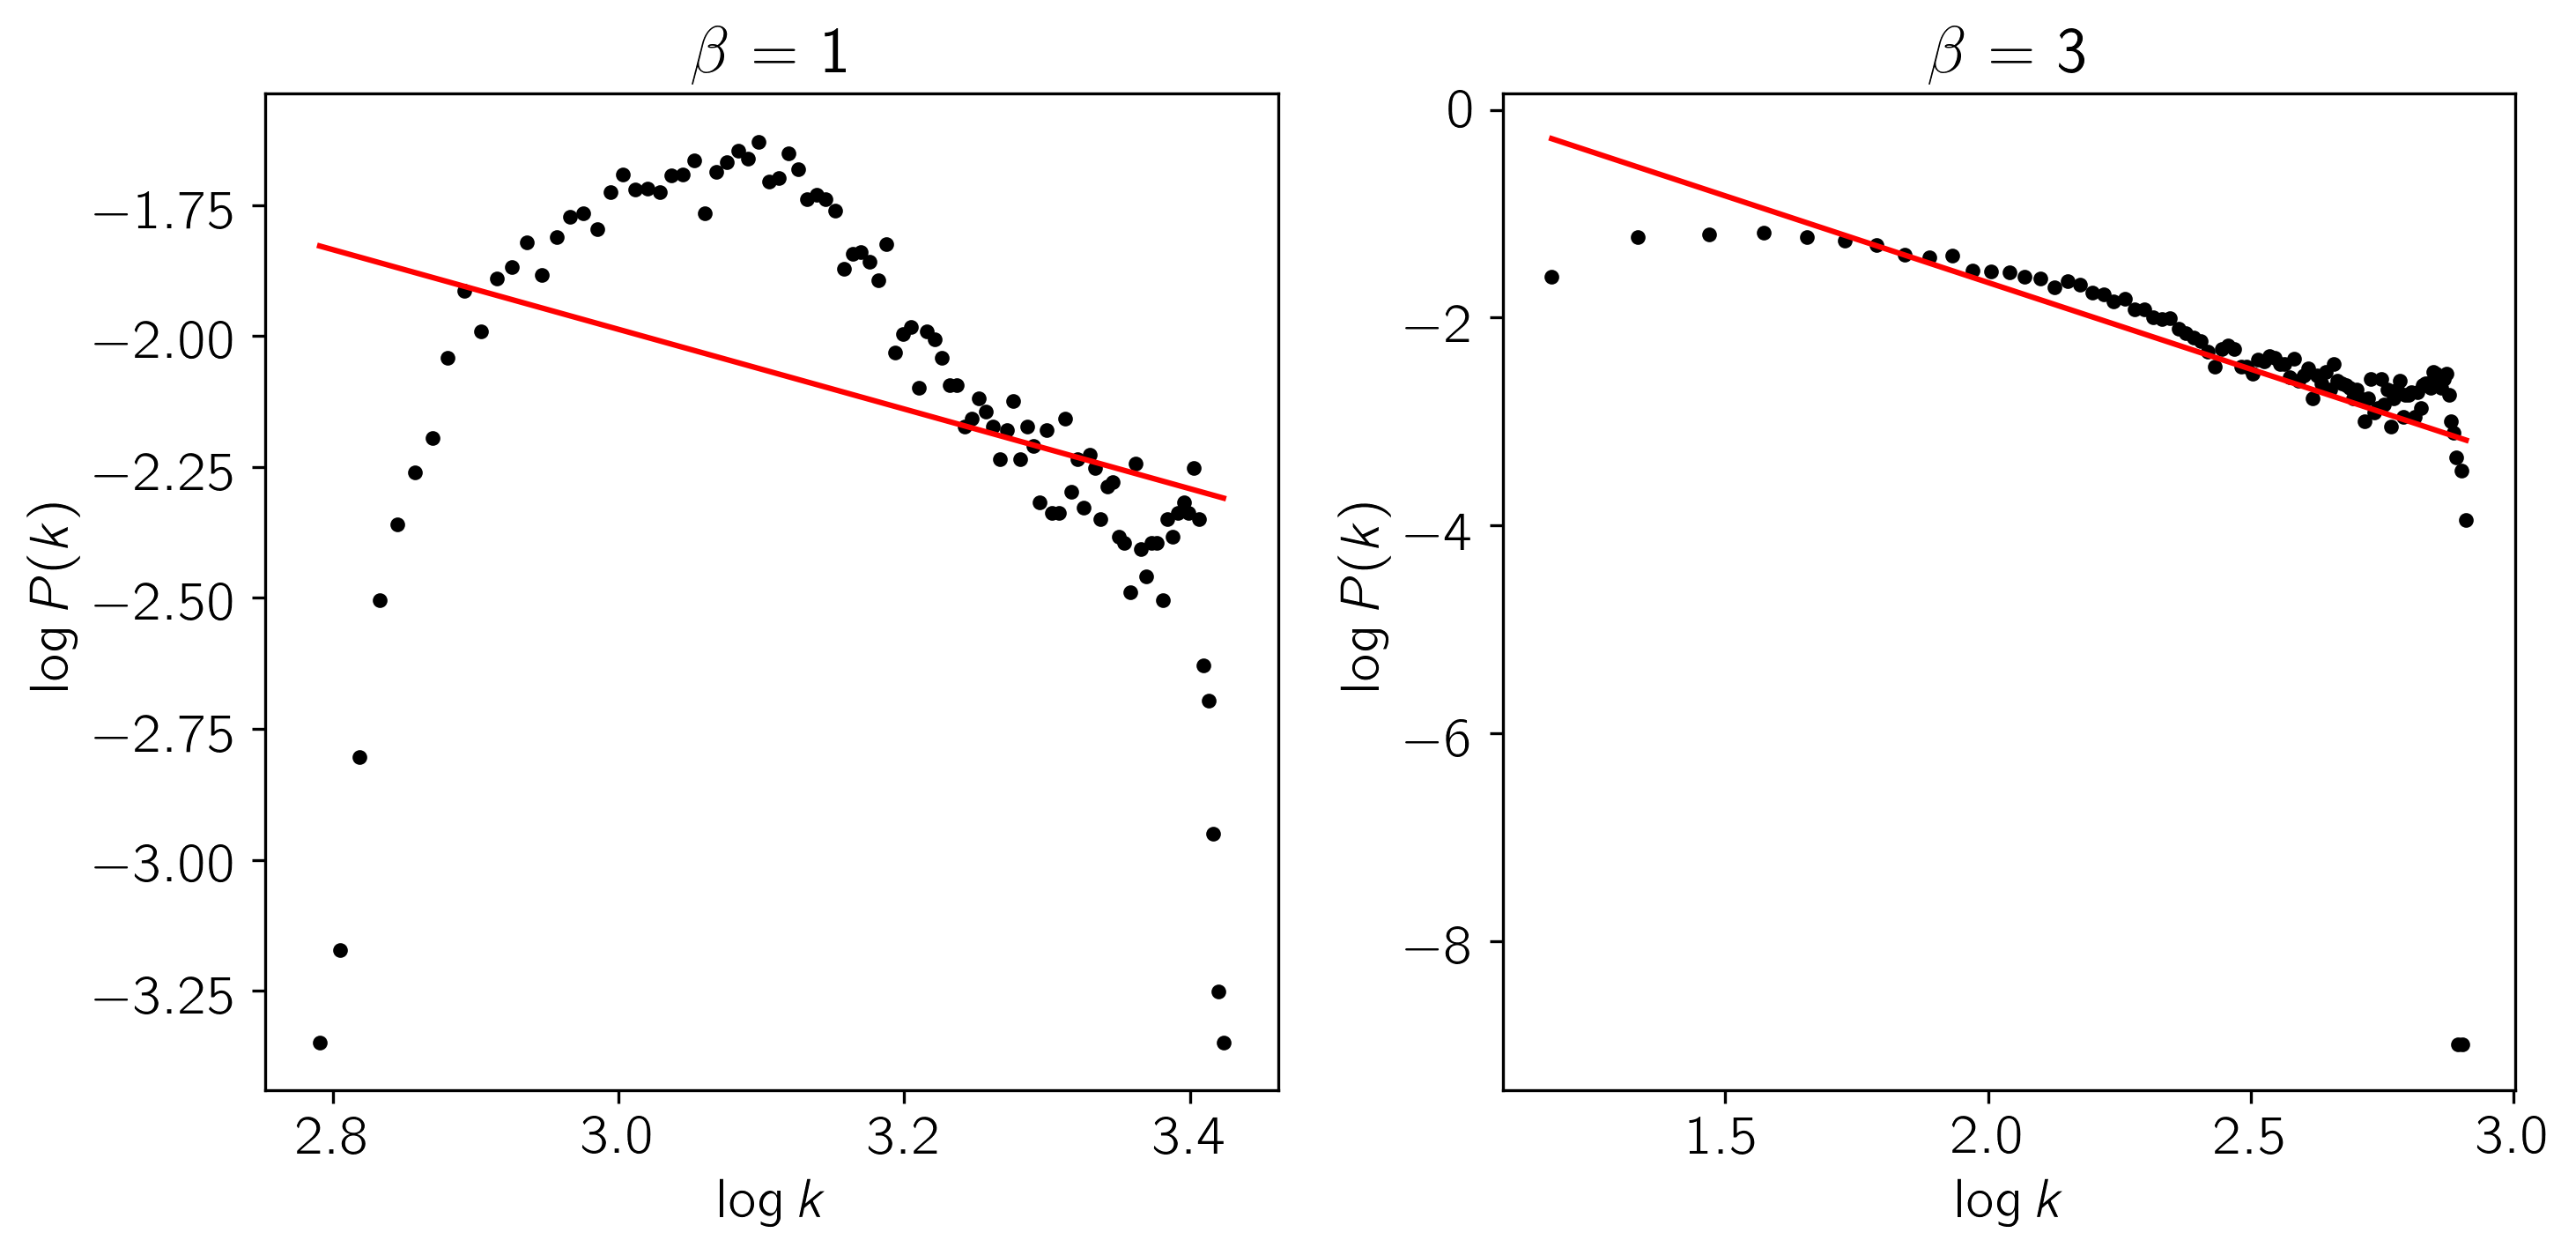
\includegraphics[clip,width=0.8\textwidth]{figures/figure2.png}
  \caption{Degree distribution of the network represented by $S$ (left) and $A$ (right).}
  \label{fig:beta}
\end{figure}

The resulting adjacency matrix $A$ represents a complete graph
$G=(V,E)$, with $|V| = 8\,928$ genes ($|E| = 39\,850\,128$ edges).

\subsection*{C. Identification of Co-expression Modules}

The adjacency matrix $A$ is transformed into an unweighted network
$\hat{A}$ applying the approach described
in~\cite{aoki2007approaches}. The cutoff value is set to $0.2$, 
based on the density of the network
combined with the decreasing number of nodes and edges with higher PCC
values. Thus keeping only the
connections above this threshold and removing any isolated nodes. The
resulting adjacency matrix $\hat{A}$ has $5\,810$ connected genes and
accounts for $614\,501$ edges.
\vspace{0.5cm}

After applying the HLC algorithm, a total of $4\,131$ genes are
distributed in $c = 5\,143$ overlapping modules of at least $3$
genes. Figure~\ref{fig:overlap} presents a histogram of the
overlapping percentage of these genes, measured as the proportion of
modules to which each gene belongs. The first bar of the histogram
represents the genes with zero overlap, corresponding to $28\%$ of the
total genes; the remaining $72\%$ represents the genes belonging to
more than one module.

%figure 3
\begin{figure}[htbp]
  \centering
    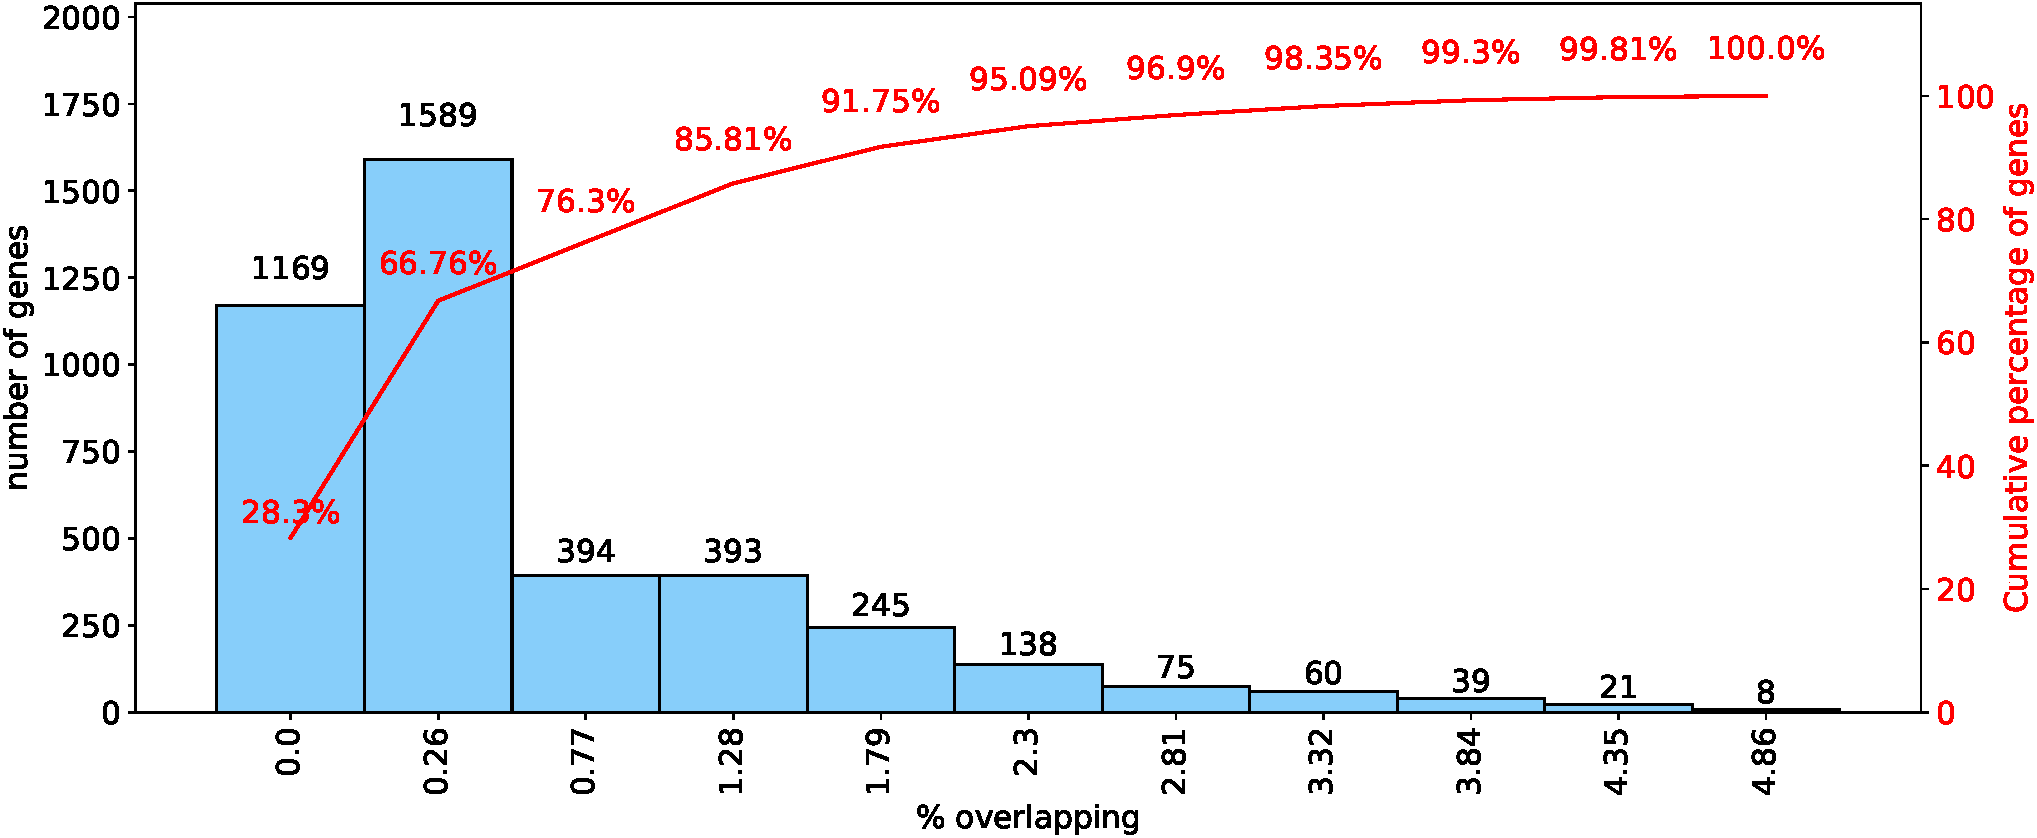
\includegraphics[clip,width=0.95\textwidth]{figures/figure3.pdf}
  \caption{Overlapping percentage of genes after applying HLC.}
  \label{fig:overlap}
\end{figure}

\subsection*{D. Detection of Modules Association to Phenotypic Traits}

The phenotypic traits under study are shoot $K$ content, root
biomass, and shoot biomass. Figure~\ref{fig:pdata} suggests that there
are significant differences in the values of these phenotypic traits
between stress and control conditions. This supports the working
hypothesis that these three variables represent tolerance-associated
traits in rice under salt stress.
\vspace{0.5cm}

%figure 4
\begin{figure}[htbp]
  \centering
    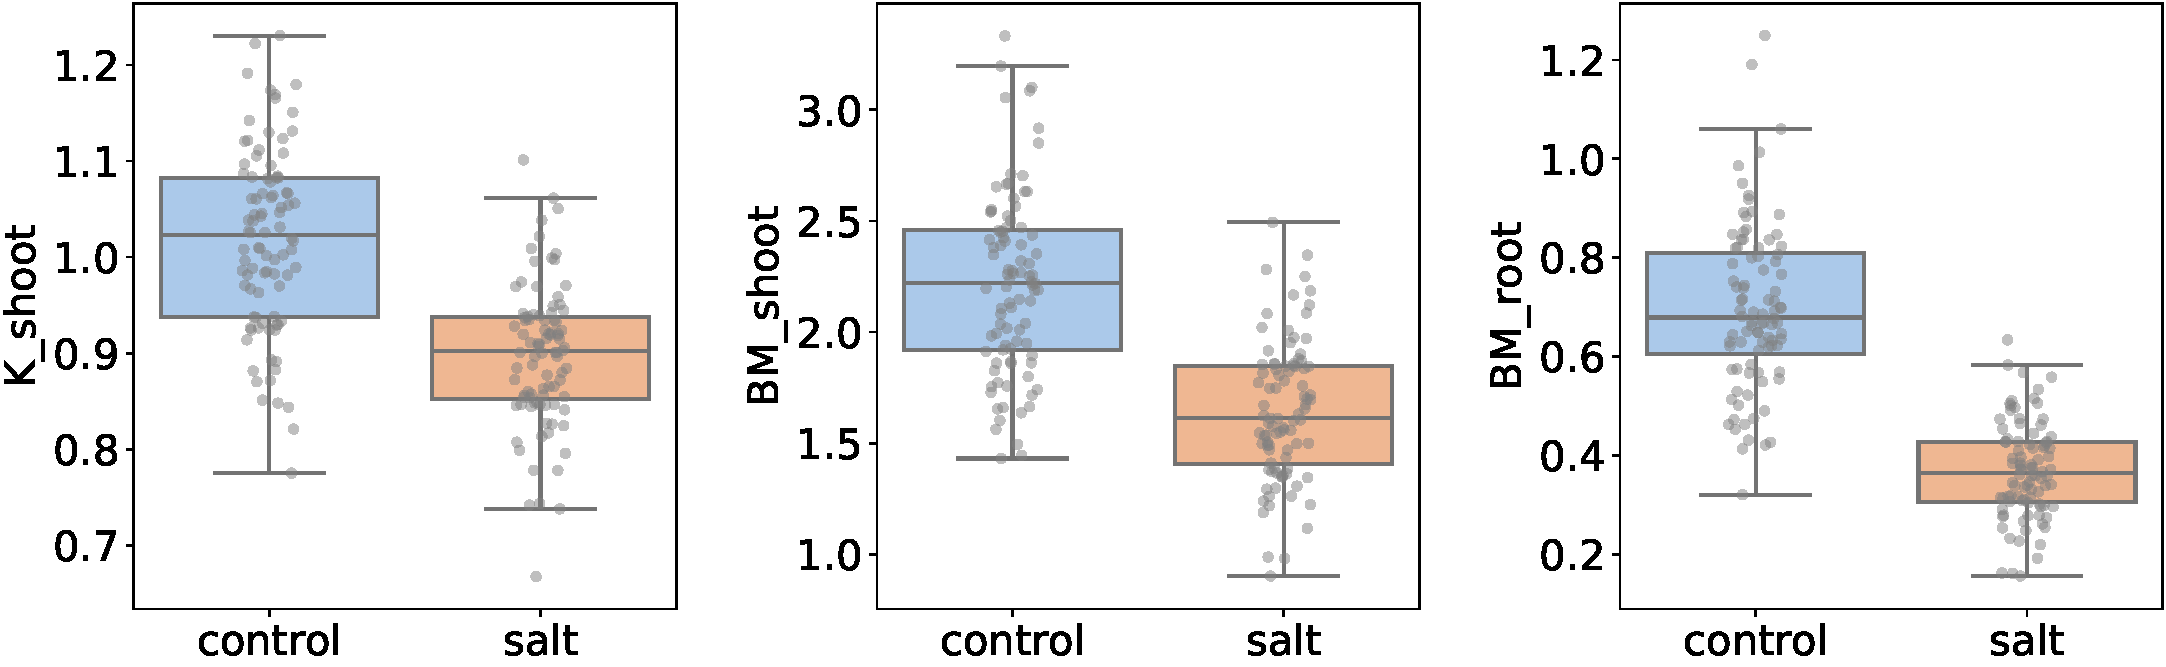
\includegraphics[clip,width=0.9\textwidth]{figures/figure4.pdf}
  \caption{Phenotipic traits distribution under control and salt stress.}
  \label{fig:pdata}
\end{figure}

Using the affiliation matrix $F$ derived from the HLC output and the
Log Fold Change matrix $L_1$, a matrix $M$ is built by computing the
eigengene for each of the $c = 5\,143$ modules. The LASSO technique is
applied by using each of the phenotypic traits as the outcome
variable, one at a time. As shown in Figure~\ref{fig:cross-val},
cross-validation is performed for each phenotypical trait in order to
select the corresponding regularization parameter $\lambda$ that
minimizes the mean-squared error.
\vspace{0.5cm}

%figure 5
\begin{figure}[htbp]
  \centering
    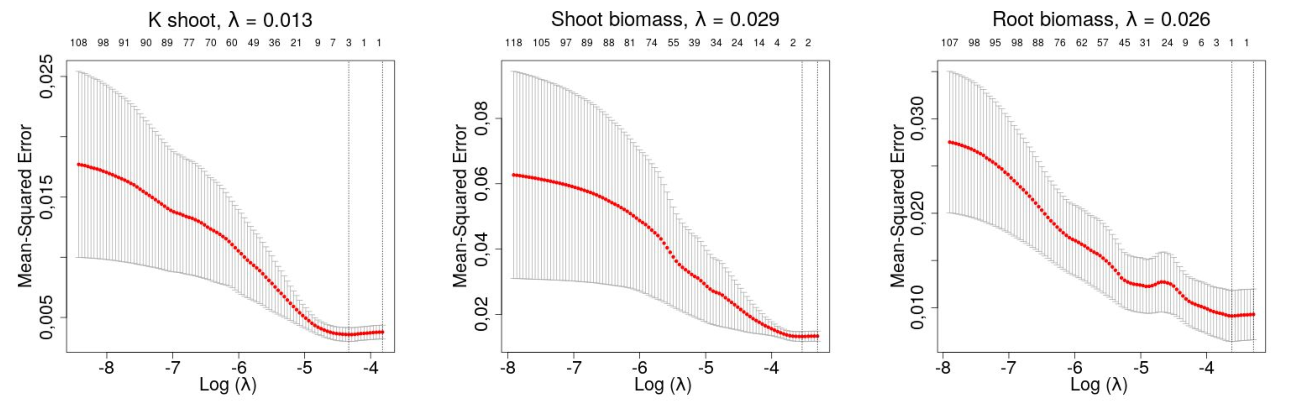
\includegraphics[clip,width=0.96\textwidth]{figures/figure5.pdf}
  \caption{Cross-validation of the LASSO regularization parameter
    $\lambda$, for each phenotypic trait.}
  \label{fig:cross-val}
\end{figure}

Finally, three LASSO models are adjusted by using the corresponding
$\lambda$ and phenotypical data with the eigengenes of matrix $M$. As
result, 6 modules are detected as relevant in the response to salt
stress in rice: 3 modules of 3 genes, each associated with shoot $K$
content; 2 modules of 3 genes associated with shoot biomass; and 1
module of 4 genes associated with root biomass (see
Figure~\ref{fig:final_genes}).

\subsection*{E. Gene Enrichment}

From the $19$ genes selected by LASSO, all but $3$ genes (the ones
associated to $K$ content), are also identified as deferentially
expressed ($|\ell_{ij}| \geq 2$) for at least one of the $92$
accessions. These genes are strong 
candidates target genes in rice.
%candidates as stress responsive genes to salt conditions in rice.
\vspace{0.5cm}

Figure~\ref{fig:final_genes} summarizes how from the initial
$n_0=57\,845$ genes, the proposed workflow identifies a reduced set of
$19$ genes. First, $48\,431$ genes are discarded after filtering the
normalized expression data $D_2$ and then $486$ additional genes are
discarded when filtering the Log Fold Change matrix $L_0$, to finally
arrive at $19$ genes, of which $16$ are differentially expressed.
\vspace{0.5cm}

% figure 6
\begin{figure}[htbp]
  \centering
    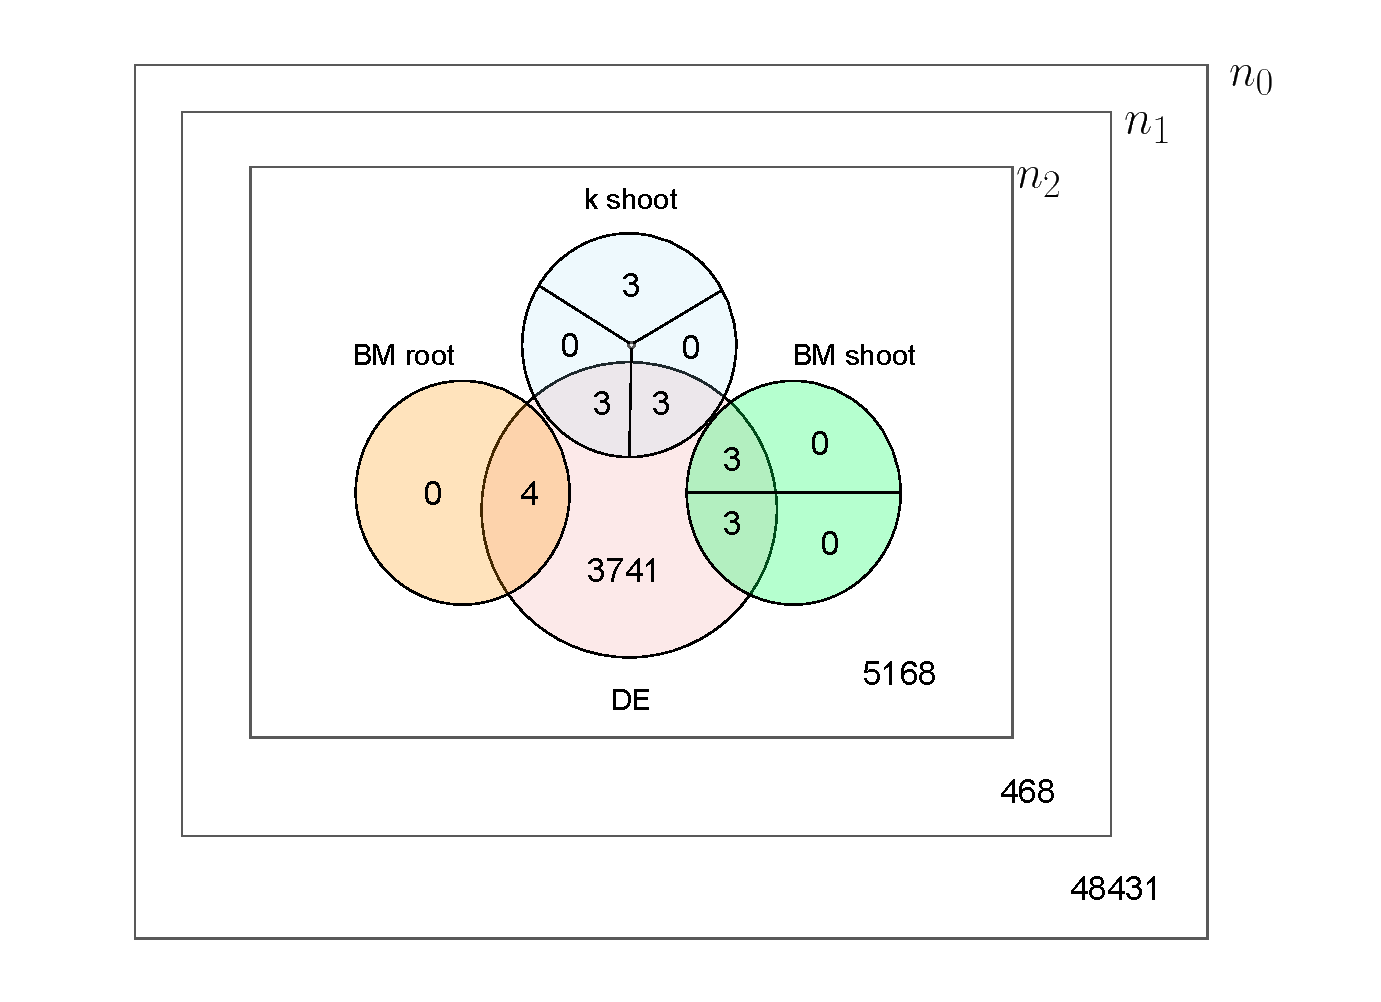
\includegraphics[clip,width=0.8\textwidth]{figures/figure6.pdf}
   \caption[Venn diagram for the case study in rice]%
   {Venn diagram representing the number of genes selected at
    different stages of the proposed workflow for the case study in
    rice.}
  \label{fig:final_genes}
\end{figure}

According to the Quickgo database, only $2$ of the $16$ differentially
expressed genes (both from the module related to shoot biomass) are
named and have an associated protein product: spermidine
hydroxycinnamoyltransferase 2 (SHT2) and lipoxygenase.
Figure~\ref{fig:3d} shows their corresponding 3D protein structures.
\vspace{0.5cm}

%figure 7
\begin{figure}[htbp]
  \centering
    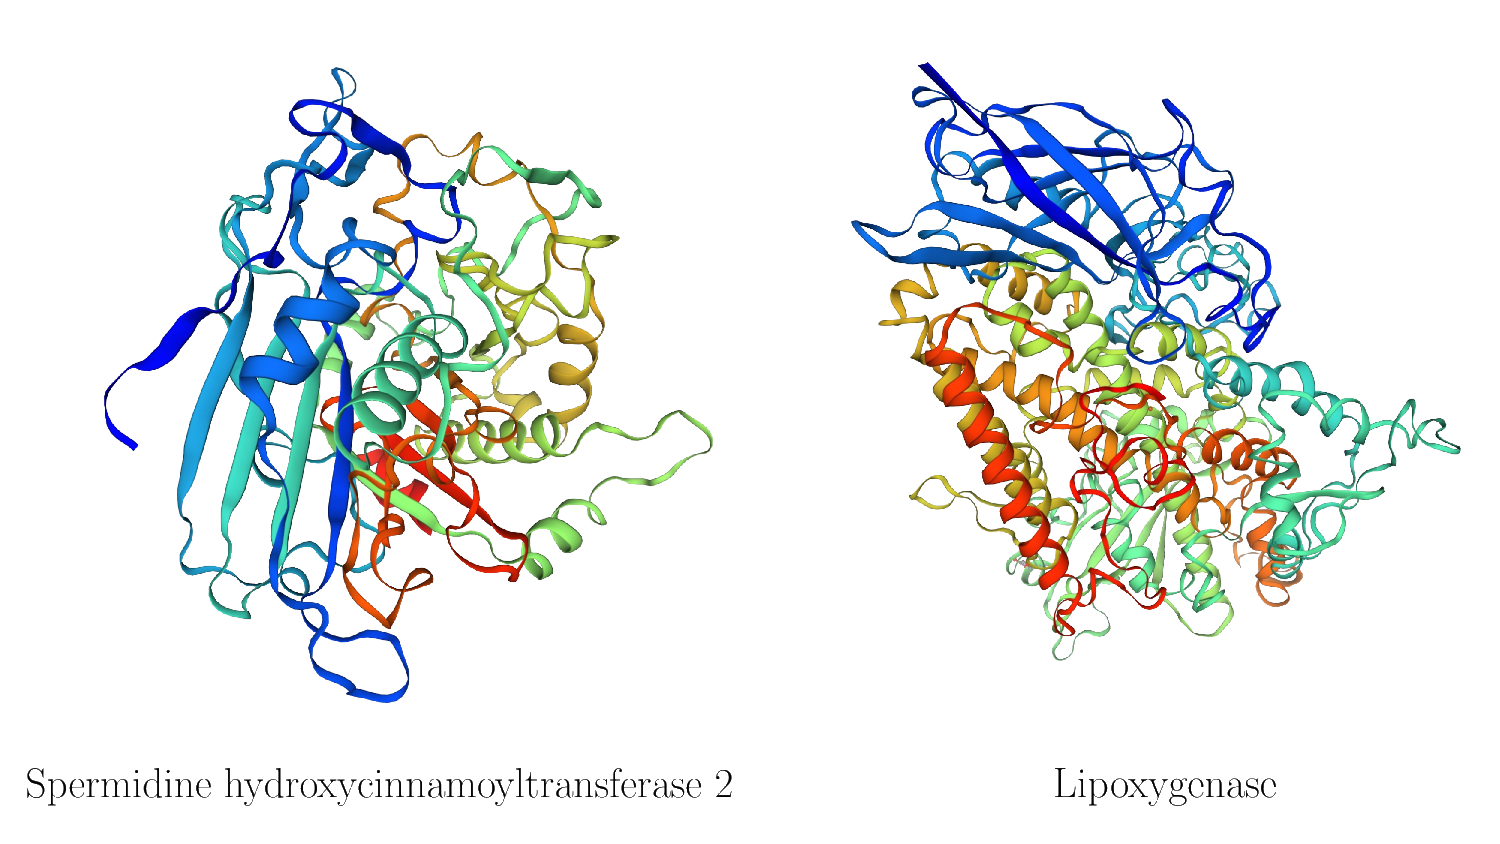
\includegraphics[clip,width=0.8\textwidth]{figures/figure7.pdf}
  \caption{3D protein structure of named genes selected by LASSO, borrowed from~\cite{szklarczyk2016string}.}
  \label{fig:3d}
\end{figure}

The Uniprot database~\cite{uniprot2018uniprot} reports, on the one
hand, that SHT2 contributes to the natural variation of
spermidine-based phenolamides in rice cultivars. On the other hand, it
is reported in~\cite{uniprot2018uniprot} that plant lipoxygenase may
be involved in a number of diverse aspects of plant physiology
including growth and development, pest resistance, and senescence or
responses to wounding. This protein is involved in the pathway
oxylipin biosynthesis, which is part of Lipid metabolism. Additionally,
previous studies
%
in~\cite{gupta2013plant,hou2015persimmon,mittova2002salt,peng2019novel,roychoudhury2011amelioration}
%
provide evidence of biological implications of sperimidine and
lipoxygenase in tolerance to salt stress in other plants or even in
rice cultivars.

As a conclusion, the results presented in this section suggest that
further studies are needed to elucidate the detailed biological
function of the remaining 14 genes that have not been named so far in
the literature.  They may have the potential to intervene in stress
responsive mechanisms to salt conditions in rice.
